\chapter{Soundness}
    \section{Soundness in Petri Nets}
    Soundness is a critical property in Petri nets, ensuring that the model behaves correctly. A Petri net is considered \textbf{sound} if it satisfies the following three conditions:
    \begin{enumerate}
        \item \textit{Option to complete:} From any reachable marking, there is a path to the final state (i.e., the process can always finish).
        \item \textit{Proper completion:} The final marking (where a token is in the output place) is the only marking where no other transitions are enabled.
        \item \textit{No dead transitions:} Every transition in the Petri net can be fired at least once during the process execution.
    \end{enumerate}
    Soundness guarantees that the process modeled by the Petri net is reliable for analysis and execution.
    
    \section{Reachability Graph}
    The \textbf{reachability graph} of a Petri net is used to show all the possible states (markings) the net can reach from its initial marking. It represents the behavior of the Petri net by enumerating all possible transitions between states.
    
    The steps to create a reachability graph are as follows:
    \begin{enumerate}
        \item Label the initial marking $m_0$ as the root and tag it as "new".
        \item While new markings exist:
        \begin{itemize}
            \item Select a new marking $m$.
            \item If no transitions are enabled at $m$, tag it as a "dead-end".
            \item For each enabled transition $t$:
            \begin{itemize}
                \item Fire the transition $t$ and obtain a new marking $m'$.
                \item If $m'$ does not already exist in the graph, add it and tag it as "new".
                \item Draw an arc from $m$ to $m'$ labeled with $t$.
            \end{itemize}
        \end{itemize}
        \item Output the reachability graph.
    \end{enumerate}
    
    \subsection{Example of Reachability Graph Construction}
    
    \begin{figure}
        \centering
        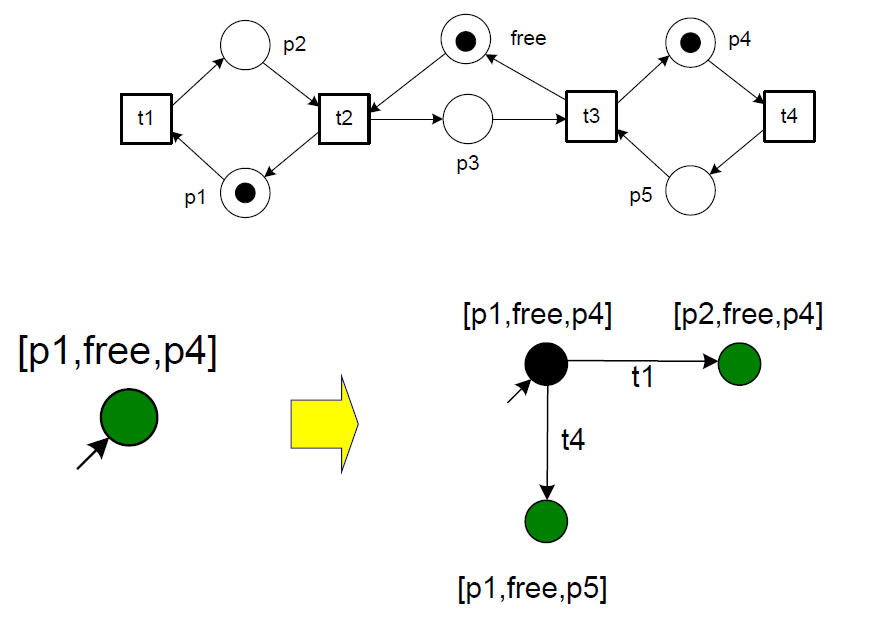
\includegraphics[width=0.5\linewidth]{capitolo 4/reachability graph 1.png}
    \end{figure}
    Let us consider an example of a simple Petri net. The following steps illustrate the process of constructing the reachability graph step-by-step. The functioning of a reachability graph is as follows. Initially, we are in the configuration \([p1, \text{free}, p4]\), where this notation indicates the places where the tokens are located. Let us assume that we \textit{fire} transition \(t1\); consequently, the new configuration will be \([p2, \text{free}, p4]\). We then draw an arrow connecting the new configurations. Obviously, the choice to fire \(t1\) instead of \(t4\), which would have led to the configuration \([p1, \text{free}, p5]\), was arbitrary. This does not matter because, when constructing the reachability graph, we must explore and study all possible cases.
    \begin{figure}[h]
        \centering
        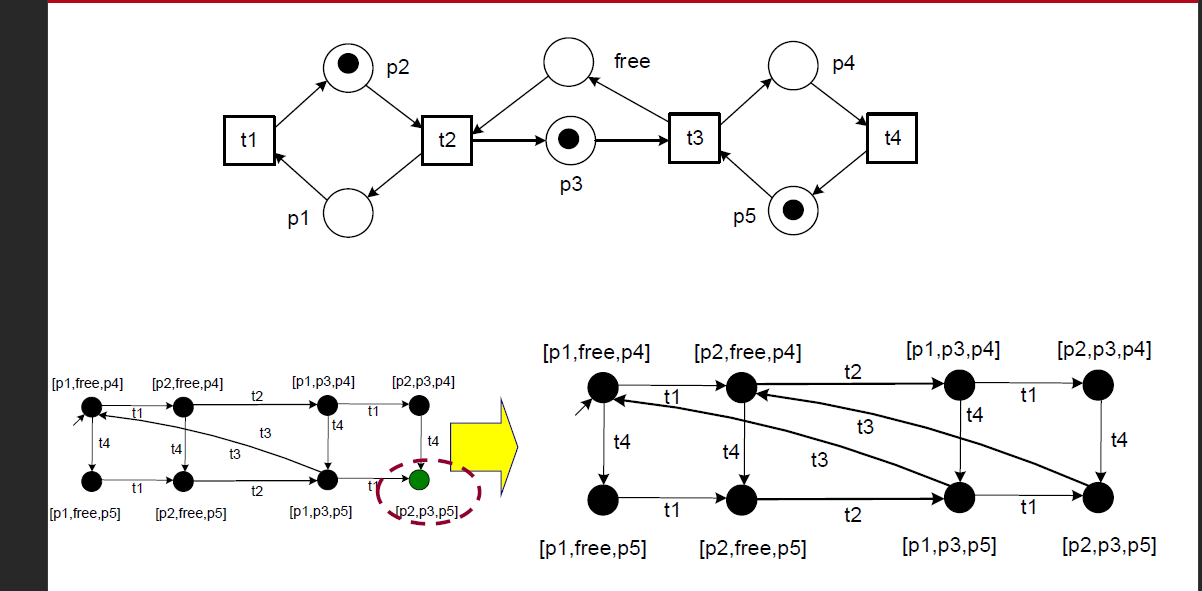
\includegraphics[width=0.8\linewidth]{capitolo 4/reachability graph 2.png}
    \end{figure}
    
    By continuing in this manner, we eventually obtain transitions that return us to the initial state, thus creating a closed and cyclic path.
    
    
    \section{Key Properties of Petri Nets}
    
    \subsection{Boundedness}
    A place in a Petri net is said to be \textbf{bounded} if there is a limit to the number of tokens it can hold. Formally, a place $p$ is $k$-bounded if $p$ can hold at most $k$ tokens, for some integer $k$.
    \begin{itemize}
        \item If $k = 1$, the place is \textit{safe}.
        \item If no such $k$ exists, the place is \textit{unbounded}.
    \end{itemize}
    Boundedness can be verified by constructing the reachability graph, as a bounded Petri net will have a finite reachability graph.
    
    \subsection{Deadlock}
    A \textbf{deadlock} occurs in a Petri net when no transitions are enabled in a particular marking. This means that the process is stuck, and no further actions can be taken. It is a marking with no enable transistions.
    
    \subsection{Dead Transitions}
    A \textbf{dead transition} is one that can never be fired in any reachable marking. Dead transitions indicate parts of the model that are unreachable during the execution of the process. They never appear in a reachability graph.
    
    \subsection{Liveness}
    A Petri net is \textbf{live} if, from every reachable marking, it is possible to fire every transition at least once in the future. \textbf{Liveness} ensures that the process can continue indefinitely without reaching a dead-end. If a net is live it cannot be dead transitions. 
    
    \subsection{Home-Markings and Reversibility}
    A \textbf{home-marking} is a marking that can be reached from any other reachable marking. A Petri net is \textbf{reversible} if its initial marking is a home-marking. Reversibility guarantees that the process can always return to its starting point. Normally the final marking of a transistion should be a home marking (if there are no deadlocks).
    
    \section{Workflow Nets}
    A \textbf{workflow net} is a special type of Petri net used to model business processes. A workflow net $N = (P, T, F)$ is defined by the following properties:
    \begin{itemize}
        \item \textbf{Object creation:} The net contains an input place $i$, such that $\bullet i = \emptyset$.
        \item \textbf{Object completion:} The net contains an output place $o$, such that $o\bullet = \emptyset$.
        \item \textbf{Connectedness:} Every node in the net is on a path from $i$ to $o$.
    \end{itemize}
    
    A workflow net is sound if it satisfies the same soundness criteria discussed earlier: option to complete, proper completion, and absence of dead transitions.
    
    \section{Soundness and Reachability Graph}
    The soundness of a workflow net can be analyzed through its \textbf{reachability graph}, which must satisfy the following criteria:
    
    \begin{enumerate}
        \item \textbf{Option to complete:} From any reachable marking $m$, it is always possible to reach the final marking $[o]$ (the output place). In terms of the reachability graph, this means that $[o]$ is a \textbf{home marking}.
        
        \item \textbf{Proper completion:} The only reachable marking containing a token in place $o$ is the marking $[o]$. In the reachability graph:
        \begin{itemize}
            \item $m(o) < 2$ for all markings $m$ in the reachability graph. there it has maximum 1 token.
            \item If $m(o) = 1$, then $m(p) = 0$ for every place $p \in P \setminus \{o\}$.
        \end{itemize}
        
        \item \textbf{Absence of dead activities:} There are no dead transitions in the net, meaning that every transition appears in the reachability graph and can be fired at least once.
    \end{enumerate}
    
    The reachability graph serves as a formal tool to verify these properties and ensure the soundness of the workflow net.
    
    \subsection{Short-Circuit Net and Soundness}
    Soundness in a workflow net can be verified by creating a \textbf{short-circuit net}, where an invisible transition is added from the output place to the input place. If the short-circuit net is both live and bounded, the original workflow net is sound.
    
    \section{Coverability Graph}
    In cases where the reachability graph contains infinitely many states, an alternative analysis can be conducted using the \textbf{coverability graph}. This graph provides a finite abstraction of the reachability graph, where places that can grow unbounded are represented using the symbol $\omega$.
    \begin{itemize}
        \item A marking $m_1$ is said to be greater than another marking $m_2$ if, for every place $p$, $m_1(p) \geq m_2(p)$.
        \item The coverability graph is constructed similarly to the reachability graph but includes the $\omega$ symbol to represent unbounded places.
    \end{itemize}
    If the coverability graph contains any $\omega$, the Petri net is unbounded. Otherwise, if the coverability graph matches the reachability graph, the net is bounded.
    
    \subsection{Algorithm for Constructing the Coverability Graph}
    The algorithm to build the coverability graph follows the same steps as the reachability graph but adds the condition that, when a marking $m'$ is greater than any previously visited marking $m''$, all places where $m'(p) > m''(p)$ are set to $\omega$.
    
    \begin{figure} [h]
        \centering
        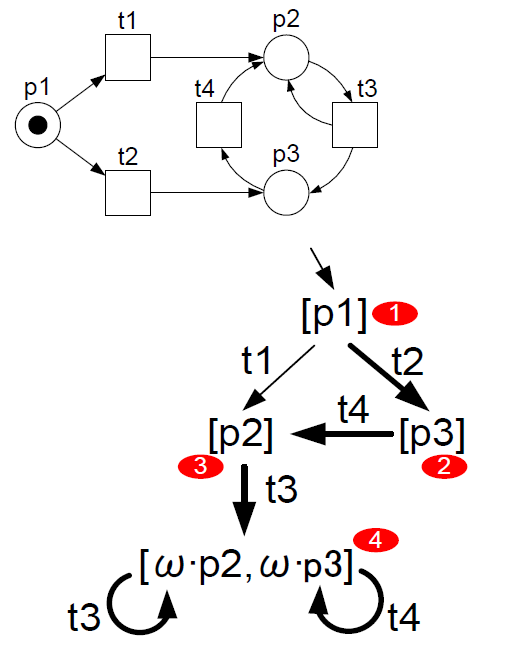
\includegraphics[width=0.5\linewidth]{capitolo 4/coverability graph.png}
    \end{figure}
    The process being described is the creation of a \textit{coverability graph}. Essentially, to represent this graph, we must base it on the rules for constructing a \textit{reachability graph}. Thus, when we start creating the graph, we explore all possible transitions that we encounter.
    
    However, if at any point (as seen in point 4 of the image) we observe that any situation has markings greater than previous ones, this means that the element is \textit{unbounded}.
    
    We see that in point 4, there are more markings on $P_2$ and $P_3$. To understand where to place the \textit{omega} ($\omega$), we need to go back. If we go back and find any marking (e.g., marking 2) that is smaller than the one we are currently at in position 4, we must place $\omega$ in the corresponding marking. 
    
    For example, in situation 4 but not in situation 3, we observe an additional marking on $P_3$, and as a result, we add $\omega$ on $P_3$. Similarly, going back from situation 4, we reach position 2, where we have an additional marking on $P_2$, so we place $\omega$ on $P_2$.
    
    Finally, we notice that from position 4 (as seen in the figure), we can apply transitions $T_3$ and $T_4$, which always lead us to similar situations. In this case, we assume $\omega = \omega + 1$ and $\omega = \omega - 1$. The exact number of $\omega$ is not relevant; what matters is that, by going to infinity, we will always encounter situations where the number of markings is greater than zero and larger than previous markings.
    
    
    
    \section{Properties of the Coverability Graph}
    \begin{itemize}
        \item The reachability graph and the coverability graph of a bounded Petri nets are equivalent.
        \item The coverability graph is always finite.
        \item A transition t of a Petri net is dead if and only if it does not appear in the coverability graph.
        \item A place p of a Petri net is k-bounded if and only if p does not contain more than k tokens in any marking of the coverability graph.
        \item Every run of a Petri net can be mimicked in the coverability graph (but not the other way around).
        \item Aplace p of a Petri net is k-bounded if and only if p does not contain more than k tokens in any marking of the coverability graph.
    \end{itemize}
    
    \section{Conclusions}
    
    Process models need to be sound in order to be useful for analysis and enactment in process-aware information systems. A model is considered sound if and only if:
    
    \begin{enumerate}
        \item It is always possible to reach a process end state (i.e., the final marking).
        \item Every process-model activity is possible, meaning there are no \textbf{dead transitions}.
        \item When the process reaches a formal end state, no further activities can be executed (i.e., no transitions can be fired).
    \end{enumerate}
    
    \newline
    \newline
    
    Petri nets provide a formal framework to conduct soundness analysis. The analysis of the \textbf{reachability graph} allows us to determine whether a Petri net-based process model is sound.
    
    \textbf{Unboundness} in the process model, indicated by the presence of the $\omega$ symbol in the \textbf{coverability graph}, signifies that the process is unsound. The coverability graph is a powerful tool for detecting unboundness, and soundness can only be guaranteed if no place in the net can grow unbounded.
    